

% Describe your planned modeling approach, 
% based on the exploratory data analysis 
% from the last two weeks (< 1 page, bullet points).


\documentclass[12pt]{article}

\usepackage{hyperref}
\author{Duncan Wood}
\title{Groove Gang Method Proposal}

\begin{document}

\maketitle

We will be performing clustering on musical recordings 
          based on their instrinsic rhythmic content.

\begin{enumerate}
\item We first use \href{https://www.github.com/mjhydri/BeatNet}{Beatnet} 
        to find a dynamic grid of beats (and downbeats) within 
        an audio track. 
\item We subdivide each measure (i.e. between downbeats) into 
        even divisions, up to some cutoff $N$, effectively 
        enumerating the rational numbers between 0 and 1.
        This gives grid timings $t_i$.
\item For the original waveform $s(t)$, compute the short-term power 
        near each subdivision $t_i$ as the weighted sum 
        $P_i = \sum_j s^2(t_j) k(t_j - t_i) $, 
        with $k$ being a gaussian kernel centered at 0, with a width
        of the hyperparameter $w$, corresponding to $\sim 30$ ms.
\item Calculate the displacement from grid $d_i$ as the distance between
        point of max power and the grid point $t_i$. 
\item Combine information for each bar into one vector as 
        $\vec{M} = (P_0, t_0, P_1, t_1, ...)$.
\item Each recording has multiple bars, so either average over bars
        or find a cluster to assign a representative rhythm for the track $\vec{T}$.
\item Compare different tracks via Euclidean distance on this encoding. 
        Cluster tracks based on this metric to find families of rhythms. 
\end{enumerate}



% \begin{figure}
% 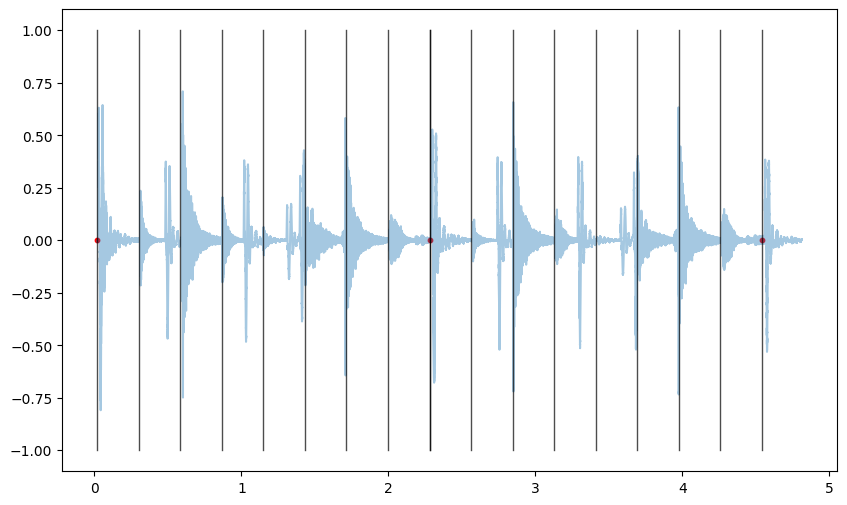
\includegraphics[]{../ims/beatnet_ex1.png}
% \end{figure}


\end{document}